%!TEX root = ../../thesis.tex
\section{WebRTC}
\label{realtime-webrtc}

WebRTC, short for Web Real-Time Communcation, is a new web communication technology that enables peer-to-peer multimedia broadcasting (audio, video and arbitrary data). It is being standardized by both the W3C\footnote{\url{http://www.w3.org/TR/webrtc}} and the IETF\footnote{\url{https://tools.ietf.org/wg/rtcweb/}} and, although it is already available in recent Chrome and Firefox versions, its API and the protocol are still in flux. The goal of WebRTC is not only to bring peer-to-peer multimedia streams to the web but also to act as a bridge technology to existing real-time applications so that browsers will be able to act as natural peers of these systems \cite[p. 310ff]{grigorik2013high}. This creates a broad spectrum of applications for WebRTC but it also renders it very complex. This section will omit many details that would be necessary to fully set up a WebRTC system but the complexity of such a system would go beyond the scope of the goal of this chapter. Therefore, it will focus on the usage of the client-side API and only briefly mention the possible network topologies and the various utilized protocols instead of explaining them all.

\begin{figure}[htb]
  \centerline{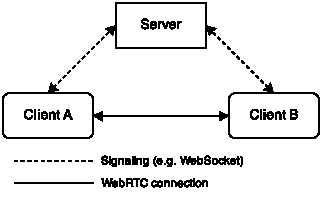
\includegraphics[width=0.9\linewidth]{images/WebRTC_connection.pdf}}
  \caption[A basic WebRTC setup]{A basic WebRTC setup}
  \label{fig:webrtc}
\end{figure}

In the most basic use case WebRTC can be used to establish a `phone' call between two parties (see \reffigure{fig:webrtc}). One of the parties (Client A) initiates this process by sending an `offer' to the other party. Since both parties are not yet connected via peer-to-peer, a signaling server is used for establishing the direct connection. Signaling includes the exchange of available codecs, security keys and addresses. The signaling process itself is, purposefully, not standardized by WebRTC because there are already several signaling protocols (e.g. SIP or Jingle) being used in existing peer-to-peer applications. WebRTC does not dictate the usage of a protocol to stay as open as possible so that a variety of applications can connect with WebRTC clients through the same protocols\footnote{\cite[p. 320ff]{grigorik2013high}}. The offer messages are sent in the SDP (Session Description Protocol) which is essentially is a pre-defined list of key-value pairs that describe the details of the session (e.g. protocol version or media description\footnote{The type of media that should be streamed to the other peer}). The other party (in this case Client B) then replies with an `answer' that is also sent in SDP format.

Once the session information has been exchanged, the parties need to connect to each other. Since most clients are connected to the Iwillwhennternet through routers that only have one public IP and handle all connected clients through NATs (Network Address Translation) with private IPs, there is no direct way to connect two clients. Therefore, in order to connect the two parties, they must also exchange their private and public IPs along with the locally associated NAT port. This is all handled in WebRTC by using the ICE (Interactive Connectivity Establishment) technique \cite[p. 50f]{johnston2012webrtc}. It uses STUN (Session Traversal Utilities for NAT) for the discovery of the public IP address and, in case STUN fails e.g. because the private addresses could not be used, it falls back on TURN (Traversal Using Relays around NAT) to establish a connection.

Many of the above mentioned protocols and negotiation flows are handled automatically by the WebRTC-related objects in the browser and only affects the implementation of signaling servers. The basic WebRTC setup shown in \reffigure{fig:webrtc} involves only the usage of \code{navigator.getUserMedia} method and the \code{RTCPeerConnection} object (see \reflisting{lst:webrtc}). \code{navigator.getUserMedia} returns streams of the requested media types and supports audio, video and screen-video. When the user has granted the usage of one of these streams, the stream can be added to a new \code{RTCPeerConnection} instance via its \code{addStream} method (line 9). As seen above, this is now the time when an offer needs to be created and sent to the other peers via the signaling service, which in this case is a simple WebSocket\footnote{The WebSocket in this example is a fictional abstraction on top of the normal WebSocket object with WebRTC-related methods suchs as \code{sendCandidate}.} connection (line 13). When a candidate for the ICE connection has been found, the candidate needs to be sent to the other peer (line 17). The \code{onicecandidate}-handler (line 21) takes care of adding ICE candidates to the \code{RTCPeerConnection} and a connection is established when both clients have successfully connected to the addresses from the ICE package. A successfully established connection triggers the \code{onaddstream} method, which gains access to the other peer's stream (line 25).

\begin{lstlisting}[language=JavaScript, caption=Connecting peers with WebRTC, label=lst:webrtc]
  var iceConfig = {"iceServers": [
    {"url": "stun:server.com:1337"}
  ]};

  var signaling = new SignalingWebSocket("/signaling");
  var peerConnection = new RTCPeerConnection(iceConfig);

  navigator.getUserMedia({"audio": true}, function(event){
    peerConnection.addStream(event.stream);

    peerConnection.createOffer(function(offer){
      peerConnection.setLocalDescription(offer);
      signaling.sendOffer(offer.sdp);
    });
  });

  peerConnection.onicecandidate = function(event){
    signaling.sendCandidate(event.candidate);
  };

  signaling.onicecandidate = function(candidate){
    peerConnection.addIceCandidate(candidate);
  };

  peerConnection.onaddstream = function(event){
    console.log(event.stream);
  };
\end{lstlisting}

In addition to media streams, WebRTC also supports a data channel (\code{RTCDataChannel}) that can send both text and binary data and that has an API similar to the WebSockets API. The data channel allows peers to send messages with even lower latency than WebSocket packages because peers are directly connected. This makes WebRTC suitable for environments that require a very low-latency package communication like collaborative editors or games\footnote{\cite[p. 109]{johnston2012webrtc}}.